% Created 2021-01-04 Mon 21:02
% Intended LaTeX compiler: pdflatex
\documentclass{scrartcl}
     \usepackage[polutonikogreek, ngerman, germanb]{babel}
     \usepackage[utf8x]{inputenc}
     \usepackage[T1]{fontenc}
     \usepackage{url}
     \usepackage{framed}
     \usepackage{ulem}
     \usepackage{reledmac}
     \usepackage{listings,xcolor}
     \usepackage{setspace}
     \usepackage{graphicx}
     \usepackage{marvosym,pifont}
     \usepackage{longtable}
     \usepackage{booktabs}
     \usepackage{hyperref}
     \usepackage[scaled=.90]{helvet}  % Helvetica für Überschriften
     \usepackage{mathptmx}            % Times für den Fließtext
     \hypersetup{unicode=false,colorlinks=true,linkcolor=blue,filecolor=cyan,citecolor=green,urlcolor=magenta}


\usepackage{fancyhdr}
\pagestyle{fancyplain}
\chead{LinguaLatina}
\lhead{KSS Latein}
\rhead{\today}
\cfoot{\thepage}
\lfoot{}
\rfoot{}
\author{Daniel Rutz}
\date{\today}
\title{Lingua Latina}
\hypersetup{
 pdfauthor={Daniel Rutz},
 pdftitle={Lingua Latina},
 pdfkeywords={},
 pdfsubject={},
 pdfcreator={Emacs 27.1 (Org mode )}, 
 pdflang={Germanb}}
\begin{document}

\maketitle


\section{Download}
\label{sec:orgc696065}
Die gesamte Homepage kann als pdf-Datei heruntergeladen werden:
\begin{itemize}
\item \href{https://www.dropbox.com/s/o6qan4c267z83ze/LinguaLatina.pdf?dl=0}{LinguaLatina.pdf}
\end{itemize}

\section{Formenlehre}
\label{sec:orge9bf09d}
Hier findest du verschiedene Übersichten über die lat. 
Formenlehre.

\begin{itemize}
\item \href{https://www.dropbox.com/s/6mg0r0cdojb8uj4/GrammaticaLatina\_Formenlehre.pdf?dl=0}{Tabellen}
\item Repetitionskarten:
\begin{itemize}
\item Verbformen im \href{https://www.dropbox.com/s/nwnbpxhokzbotzx/RepetitionskartenFormellehreLateinIndikativ.pdf?dl=0}{Indikativ}
\item Verbformen im \href{https://www.dropbox.com/s/rew7e8ofvfnxeup/RepetitionskartenFormellehreLateinKonjunktiv.pdf?dl=0}{Konjunktiv}
\item \href{https://www.dropbox.com/s/pxnj7f8e4cacyuv/RepetitionskartenFormellehreLateinPronomina.pdf?dl=0}{Pronomen}
\end{itemize}
\end{itemize}

\section{Kasuslehre}
\label{sec:org2922b9e}
Das Latein teilt mit dem Deutschen wegen seiner indogermanischen
Verwandtschaft weite Bereiche in der Kasuslehre, d.h.:
Kasusfunktionen, wie wir sie im Deutschen kennen, kommen auch im
Latein vor. Allerdings gibt es auch eine Reihe von Situationen, wo der
Gebrauch abweicht. Solche Abweichungen werden in den unten stehenden
Übungssätzen thematisiert. 

\begin{quote}
Das wichtigste der lat. Kasuslehre ist auf den folgenden Blättern
zusammengestellt:

\begin{enumerate}
\item Nominativ (Der Nominativ dient zu 99.99\% als Subjekt.)
\item \href{https://www.dropbox.com/s/u58tqi635cecqop/Genitiv.pdf?dl=0}{Genitiv}
\item \href{https://www.dropbox.com/s/5840ago7l6yus57/Dativ.pdf?dl=0}{Dativ}
\item \href{https://www.dropbox.com/s/jkexxtwk9vcq9x4/Akkusativ.pdf?dl=0}{Akkusativ}
\item \href{https://www.dropbox.com/s/lqshx110lt0ktyn/Ablativ.pdf?dl=0}{Ablativ}
\end{enumerate}
\end{quote}



\begin{itemize}
\item \href{https://www.dropbox.com/s/akc5ni1scwurcft/Akkusativ\_Dativ.pdf?dl=0}{Übungssätze} zum Akkusativ und Dativ (\href{https://www.dropbox.com/s/84atgr40hz3of1y/Akk\_Dat.pdf?dl=0}{Wortangaben})
\item \href{https://www.dropbox.com/s/y8u45qf1ejjlyyh/Genitiv\_Ablativ.pdf?dl=0}{Übungssätze} zum Genitiv und Ablativ (\href{https://www.dropbox.com/s/jh8hztx21svu1rn/Wortangaben\_Genitiv\_Ablativ.pdf?dl=0}{Wortangaben})
\end{itemize}

\section{Satzlehre}
\label{sec:orgc141ca4}
Die Satzlehre beschreibt den Bau von Sätzen, die Satzarten und
Satzglieder. In der lat. Grammatik verwenden wir für die Darstellung
der Satzglieder das sog. "`Satzmodell"'.

\begin{center}
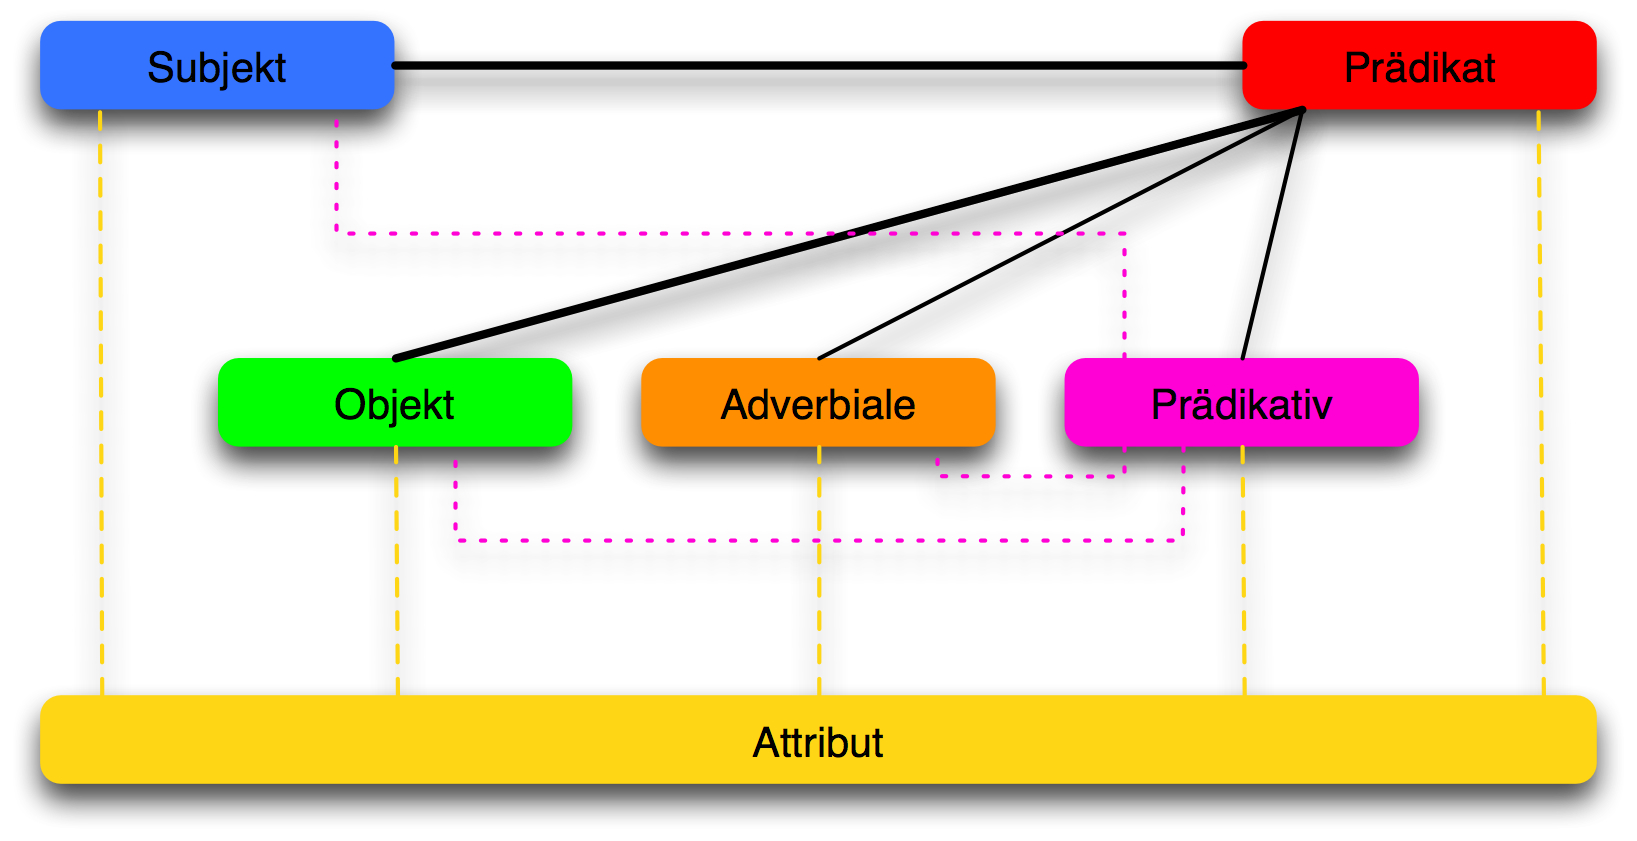
\includegraphics[width=.9\linewidth]{satzmodellfarbig.jpg}
\label{orgf385e31}
\end{center} 

\{\{< alert style="`info"' >\}\}
Erläuterungen zum Satzmodell, besonders was alles Subjekt, Objekt
etc. sein kann, findest du in \href{https://www.dropbox.com/s/id081k5itrib85b/Z19\_Satzmodell.pdf?dl=0}{diesem Dokument}.
\{\{< /alert >\}\}

In der Regel kommt bereits ein mässig komplizierter Satz als
Satzgefüge (d.h. Haupt- und Nebensätze in einem Satz) daher. In der
Grammatik werden Hauptsätze und Nebensätze getrennt behandelt.

\subsection{Besonderheiten im Hauptsatz}
\label{sec:orgb034a43}

Man kann die Hauptsätze gemäss den Satzzeichen (.?!) in drei Gruppen
einteilen:

\begin{center}
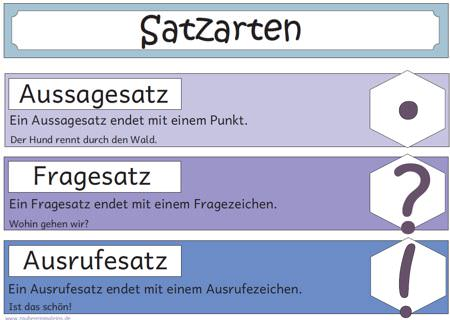
\includegraphics[width=.9\linewidth]{satzarten.jpg}
\label{org2ee0982}
\end{center}

\{\{< alert style="`info"' >\}\}
Weitere Informationen zu den Satzarten findest du in \href{https://www.dropbox.com/s/fskiu3e5rj485xp/Satzgrammatik.pdf?dl=0}{diesem Dokument}.
\{\{< /alert >\}\}

\subsubsection{Konjunktiv im Hauptsatz}
\label{sec:org929bdc1}

\{\{< panel title="`NOTA BENE!"' style="`primary"' >\}\} Der Gebrauch des lat. Konjunktivs im Hauptsatz ist anspruchsvoll,
weil er sich in einigen Bereichen nicht mit dem Gebrauch des
dt. Konjunktivs deckt. \href{https://www.dropbox.com/s/k03cq5ysu5of1ha/KonjunktivHS.pdf?dl=0}{Diese Übersicht} soll das Übersetzen des
lat. Konjunktivs, der in lat. HAUPTSÄTZEN steht, erleichtern. Die
Übersicht orientiert sich an den Satzzeichen (.?!):
\{\{< /panel >\}\}


\begin{center}
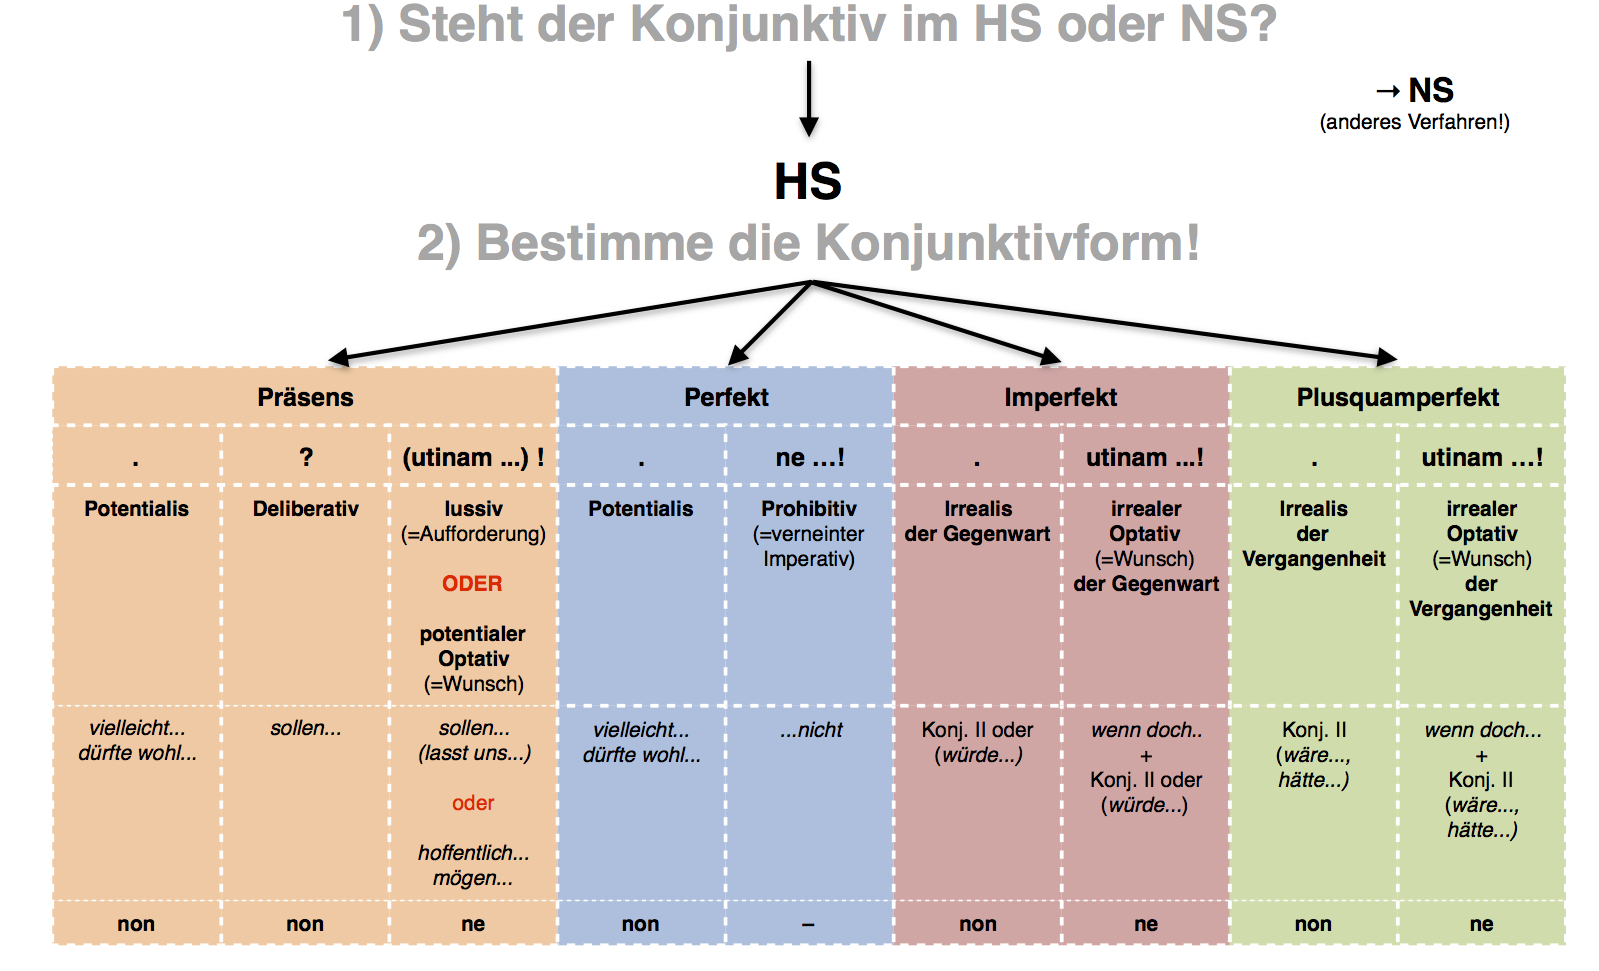
\includegraphics[width=.9\linewidth]{KonjHS.jpg}
\label{orgfaf7928}
\end{center} 

\begin{itemize}
\item \href{https://www.dropbox.com/s/sltkmozc04i5xwl/Konjunktiv.pdf?dl=0}{Übungssätze} mit Lösung und \href{https://www.dropbox.com/s/uicgeuj6n24kj97/Konjunktiv\_Wortangaben.pdf?dl=0}{Wortangaben} zum lat. Konjunktiv im
Hauptsatz.
\end{itemize}


Die einzelnen Konjunktivfunktionen müssen nicht auswendig gelernt werden.
Allerdings wird die Kenntnis der Terminologie und deren Bedeutung verlangt.


\subsection{Besonderheiten im Nebensatz}
\label{sec:org83cbee2}


\{\{< alert style="`info"' >\}\} Grundlegendes zu den lat. Nebensätzen findest du in \href{https://www.dropbox.com/s/fw6yy5i00lxn5iy/Lat\_Nebens\%25C3\%25A4tze.pdf?dl=0}{diesem Dokument}. \{\{< /alert >\}\}



Ein Merkmal lat. Nebensätze ist, dass das Prädikat oft im Konjunktiv
steht (aber nicht immer!). Dieser Konjunktiv im NEBENSATZ muss beim
Übersetzen ins Deutsche \uline{meistens} nicht mit einem deutschen Konjunktiv
wiedergegeben werden, ausser bei si-Sätzen (Wenn sie potential oder irreal sind.).

\subsubsection{Adverbiale Nebensätze}
\label{sec:org3888234}

\begin{itemize}
\item Besondere "`\href{https://www.dropbox.com/s/qundz0kc7wi3sp0/grammatik.pdf?dl=0}{Schmankerl}"' der lat. Nebensatzlehre mit
\href{https://www.dropbox.com/s/rv0zs8gtuk155ho/Grammatikrepetition\_\%25C3\%259Cbersetzung.pdf?dl=0}{Übersetzung}. Folgende Themen werden behandelt:
\begin{itemize}
\item ut-Sätze
\item cum-Sätze
\item si-Sätze
\end{itemize}
\item \href{https://www.dropbox.com/s/smmjy9k0a33qfwm/\%25C2\%25A751ut.pdf?dl=0}{ut-Sätze} (Übungssätze, Wortangaben, Lösungen in einem Dokument)
\end{itemize}

\subsubsection{Relativsätze}
\label{sec:org51fb321}

\begin{itemize}
\item \href{https://www.dropbox.com/s/60ggp3yeav4ofe8/Relativs\%25C3\%25A4tze.pdf?dl=0}{Übungssätze}; \href{https://www.dropbox.com/s/ipz22adwi00i8o8/\%25C2\%25A747Relativs\%25C3\%25A4tze.pdf?dl=0}{Wortangaben}; \href{https://www.dropbox.com/s/fttk7f0dwqlrag9/Relativs\%25C3\%25A4tze\_L\%25C3\%25B6sung.pdf?dl=0}{Lösungen}
\item \href{https://www.dropbox.com/s/xxtjdft670v04y2/Relativsatz.pdf?dl=0}{Übungssätze} (mit Wortangaben und Lösungen)
\end{itemize}

\section{Satzwertige Konstruktionen}
\label{sec:org498e56b}
Eine satzwertige Konstruktion ist eine lateinische Konstruktion, die
im Deutschen oft mit einem Satz (Haupt- oder Nebensatz) übersetzt
wird.

Folgende lat. Konstruktionen gelten als satzwertig:

\begin{enumerate}
\item Partizipialkonstruktionen
\begin{enumerate}
\item participium coniunctum (p.c.)
\item ablativus absolutus (abl.abs.)
\end{enumerate}
\item Infinitivkonstruktionen
\begin{enumerate}
\item accusativus cum infinitivo (AcI)
\item nominativus cum infinitivo (NcI)
\end{enumerate}
\item nd-Formen (Gerundialia)
\begin{enumerate}
\item Gerundium
\item Gerundiv
\end{enumerate}
\end{enumerate}


\{\{< alert style="`info"' >\}\}Grundlegende Erläuterungen zu den satzwertigen Konstruktionen findest du in \href{https://www.dropbox.com/s/k0ti2cgg8m66et7/Satzwertige\_Konstruktionen.pdf?dl=0}{diesem Dokument}.\{\{< /alert >\}\}

\subsection{Bemerkungen zur Terminologie}
\label{sec:orge35db90}

In den gängigen Grammatiken kommen Bezeichnungen wie "`Infinitiv Präsens aktiv"', "`Partizip Perfekt passiv"' usw. vor. Ich finde diese Bezeichnungen nicht ideal, da "`Präsens"' und "`Perfekt"' bei der Bezeichnung von Infinitiven und Partizipien kein absolutes, sondern (nur) ein relatives Tempus bezeichnen. Je nach Zeitverhältnis müssen diese Inifinitve und Partizipen im Deutschen gerade nicht mit Präsens oder Perfekt übersetzt werden. Ich wähle die folgenden Terminologie:

\subsubsection{Infinitive}
\label{sec:org8be1015}

\begin{center}
\begin{tabular}{lll}
 & aktiv & passiv\\
vz & AIV & PIV\\
gz & AIG & PIG\\
nz & AIN & PIN\\
\end{tabular}
\end{center}


\{\{< alert style="`warning"' >\}\} Bsp.: AIV = aktiver Infinitv der Vorzeitigkeit \{\{< /alert >\}\}


\begin{center}
\begin{tabular}{lll}
AIV & laudavisse, vidisse, audivisse, petivisse, cepisse & Perfst.+isse\\
PIV & laudatum esse, visum esse, \ldots{} & PPV (Nom.Sg.n.)+esse\\
AIG & laudare, vidêre, audire, petere, capere & Infektst.+(e)+re\\
PIG & laudari, videri, audiri, peti, capi & Infektst.+ri / Infektst.+i\\
AIN & laudaturum esse, visurum esse, \ldots{} & APN (Nom.Sg.n.)+esse\\
PIN & laudatum iri, visum iri, \ldots{} & PPV (Nom.Sg.n.)+iri\\
\end{tabular}
\end{center}


\{\{< panel title="`NOTA BENE!"' style="`primary"' >\}\} Im PIV und AIN kongruiert das Partizip z.B. im AcI mit dem Subjektsakkusativ. (Im PIN nie!) \{\{< /panel >\}\}



\subsubsection{Partizpien}
\label{sec:orgdb1a467}

\begin{center}
\begin{tabular}{lll}
 & aktiv & passiv\\
vz & (APV nur Deponens) & PPV\\
gz & APG & ---\\
nz & APN & ---\\
\end{tabular}
\end{center}

\{\{< panel title="`NOTA BENE!"' style="`primary"' >\}\} Das Partizip der Vorzeitigkeit der Deponentien sieht formal wie ein PPV aus, wird aber aktivisch übersetzt. Passive Partizipen für die Gleichzeitigkeit und Nachzeitigkeit gibt es nicht. \{\{< /panel >\}\}

\begin{center}
\begin{tabular}{ll}
APV = PPV & laudatus, a, um \ldots{}\\
APG & laudans, laudantis \ldots{}\\
APN & laudaturus, a, um \ldots{}\\
\end{tabular}
\end{center}


\{\{< panel title="`NOTA BENE!"' style="`primary"' >\}\} PPV und APN werden nach der a-/o-Deklination dekliniert, das APG folgt der konsonantischen Deklination. \{\{< /panel >\}\}

\subsection{Partizipialkonstruktionen}
\label{sec:orge622d40}

\begin{itemize}
\item \href{https://www.dropbox.com/s/7hgaz2130uzlw0d/\%25C2\%25A746Partizipialkonstruktionen.pdf?dl=0}{Partizipialkonstruktionen} (Übungssätze, Wortangaben, Lösungen in
einem Dokument)
\item \href{https://www.dropbox.com/s/9uwdu2l7g1kr8gi/PC\_ablabs2.pdf?dl=0}{p.c. und abl.abs.} (Übungssätze mit Lösungen)
\end{itemize}

\subsection{AcI}
\label{sec:org3a33991}

\begin{itemize}
\item \href{https://www.dropbox.com/s/p3vtu5snnd3z27r/AcI.pdf?dl=0}{Übungssätze} (mit Wortangaben und Lösungen)
\item \href{https://www.dropbox.com/s/4vx8vgcisfx9wll/AcI\_NcI.pdf?dl=0}{Übungssätze} zum AcI und NcI mit Lösungen (\href{https://www.dropbox.com/s/ef0rmrd1262svd3/Wortangaben\_AcI\_NcI.pdf?dl=0}{Wortangaben})
\end{itemize}

\subsection{nd-Formen}
\label{sec:org8d437d3}

\begin{itemize}
\item \href{https://www.dropbox.com/s/ykmw8sncd4x5gly/nd-Formen\_Rep.pdf?dl=0}{Übungssätze} mit Lösungen (\href{https://www.dropbox.com/s/psg50w3n8azfi13/Wortangaben\_nd-Formen.pdf?dl=0}{Wortangaben})
\end{itemize}

\section{Grundwortschatz (adeo 500)}
\label{sec:org344562b}
\begin{itemize}
\item \href{https://quizlet.com/class/1319955/}{quizlet-sets} für die 500 häufigsten lat. Wörter
\item die 500 häufigsten Wörter als \href{https://www.dropbox.com/s/v7m335rmadbrobt/500vocabula.pdf?dl=0}{pdf-Datei}
\end{itemize}

\section{Übersetzen mit Methode (ÜmM)}
\label{sec:org364c73a}
\begin{quote}
Nicht nur Wörter und Sätze sind Thema der Grammatik, sondern auch der Text selbst. Hinweise zur Textgrammatik findest du in \href{https://www.dropbox.com/s/fbswvhejksw6kl6/pronomina.pdf?dl=0}{diesem Dokument}.
\end{quote}

\subsection{Wörterbuch}
\label{sec:org921034b}
Als online-Wörterbuch empfehle ich \url{https://navigium.de/latein-woerterbuch.html}.

\subsection{Poesie}
\label{sec:org08a901e}
\begin{enumerate}
\item Catull, \href{https://www.dropbox.com/s/kc2coqw11nfxyj1/Catull72.pdf?dl=0}{carmen 72} (\href{http://www.gottwein.de/Lat/catull/catull072.php}{Übersetzung})
\item Ovid, Apollo und Daphne (\href{https://www.dropbox.com/s/g60dha8uuh5h0po/OVIDApolloDaphne.pdf?dl=0}{Text mit Wortangaben}; \href{https://www.dropbox.com/s/366v4v48njyzebm/\%25C3\%259CApollDaphne.pdf?dl=0}{Übersetzung})
\end{enumerate}

\subsection{Prosa}
\label{sec:org26a2877}
\begin{enumerate}
\item Cicero, Verres in Henna (\href{https://www.dropbox.com/s/gqrgxo7yjxglmdv/Matura\_LatInt\_schriftlich\_2016.pdf?dl=0}{Text}; \href{https://www.dropbox.com/s/h6y42hky2w0o2x9/\%25C3\%259Cbersetzung.pdf?dl=0}{Übersetzung})
\item Cicero, Sonderstellung des Menschen in der Welt (\href{https://www.dropbox.com/s/22oxzqeor9vqb67/LatIntSchriftlMatura2009.pdf?dl=0}{Text}; \href{https://www.dropbox.com/s/ieihesw9h0rkejd/\%25C3\%259CbersetzungMaturaLatIntensiv2009.pdf?dl=0}{Übersetzung})
\item Matura 2009 (\href{https://www.dropbox.com/s/fnt9bzwl6hklwv6/SPFSchriftlich2009.pdf?dl=0}{Text und Aufgaben}; \href{https://www.dropbox.com/s/hh89pcj1sy28kby/KorrekturSchriftlMaturaSPF2009.pdf?dl=0}{Übersetzung und Lösungen})
\item Matura 2015 (\href{https://www.dropbox.com/s/hl878959yooat32/Voki.pdf?dl=0}{Lernvokabular}; \href{https://www.dropbox.com/s/8qaeceb1qyemfwz/KSS\_Matura2015\_final.pdf?dl=0}{Text und Aufgaben}; \href{https://www.dropbox.com/s/xwvzrif0nu15j8h/Korrketur\_SPF\_Latein\_2015.pdf?dl=0}{Übersetzung und
Lösungen})
\end{enumerate}
\end{document}
